\chapter{Introduction} \label{ch:introduction}

At extreme temperatures and pressures, like those found in the very early universe and in particle colliders, quarks and gluons are no longer confined as hadrons. Instead, they form a new state of matter called the quark-gluon plasma (QGP). The QGP is a hot, dense, and strongly interacting fluid in which free quarks and gluons are the relevant degrees of freedom. This form of matter is very short-lived, only around 10 fm/c, or $10^{-23}$ seconds. It is impossible to measure the QGP with external probes due to this short lifetime, so we must use an internal probe. In all particle collisions, it is possible for a hard scattering to occur, where two partons from the colliding particles interact at a high momentum transfer, $Q^2$. The resulting particle shower is called a jet. This is one of the earliest processes to occur in the collision, and the resulting partons interact with the QGP as they traverse it and form a jet. Partons interacting with the QGP will lose energy to the medium resulting in a softer jet than if it had been produced in a vacuum. By comparing the properties of jets measured in proton-proton collisions to those measured in heavy ion collisions we can understand not only the properties of the QGP, but also the processes that occur during the evolution of the collision. In this thesis, we study the modifications to hadronization in jets produced in heavy ion collisions.

\section{QGP}

Quantum-Chromodynamics (QCD) is the mathematical theory governing the strong interaction, whose fermions are the six quarks, mediated by the eight gluons. Each quark has a color charge, either red, green, or blue, and gluons mediate interactions between pairs of color charges. Quarks are almost always bound as hadrons, comprised of either two or three quarks called mesons and baryons respectively. This is due to one of the properties of QCD called confinement, referring to the inability to isolate a color charge. Confinement arises from the fact that the strength of the strong force increases as the separation between quarks increases, up to the nucleon separation distance, and the energy required to separate them is enough to produce a new quark pair. On the other hand, as the separation between quarks decreases the strong force decreases. This phenomenon is referred to as asymptotic freedom and allows for the use of perturbative techniques to calculate the properties of QCD at short distance scales. These ideas are represented in Figure~\ref{fig:strong_force}.

\begin{figure}
    \centering
    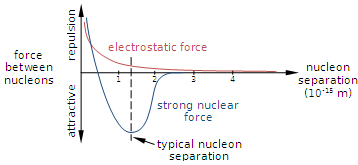
\includegraphics[width=0.8\textwidth]{figures/png/strong_force.png}
    \caption{The strong force as a function of distance compared with the electrostatic force.}\label{fig:strong_force}
\end{figure}

The QCD phase diagram is shown in Figure~\ref{fig:phase_diagram}. At high temperatures and densities, a phase transition is predicted from confined, hadronic QCD matter to a deconfined QCD matter called the quark-gluon plasma. There is an abundance of evidence for this phase transition, and the existence of a QGP, from numerical lattice QCD calculations and myriad experimental measurements[Citation needed]. The QGP forms around a termperature of 156 MeV~\cite{QCDTemp} and an energy density of around 1GeV/$fm^3$. Remarkably, the QGP behaves like a perfect liquid, which is a fluid with zero viscosity. Because of this, the QGP exhibits collective behavior like flow. Flow is the hydrodynamic evolution of pressure gradients arising from spatial anisotropies in the initial stages of the collision. Additionally, the QGP is opaque to jets, which lose energy as they traverse the medium. This phenomenon is called jet quenching and is one of the most important probes of the QGP[Citation needed]. 

\begin{figure}
    \centering
    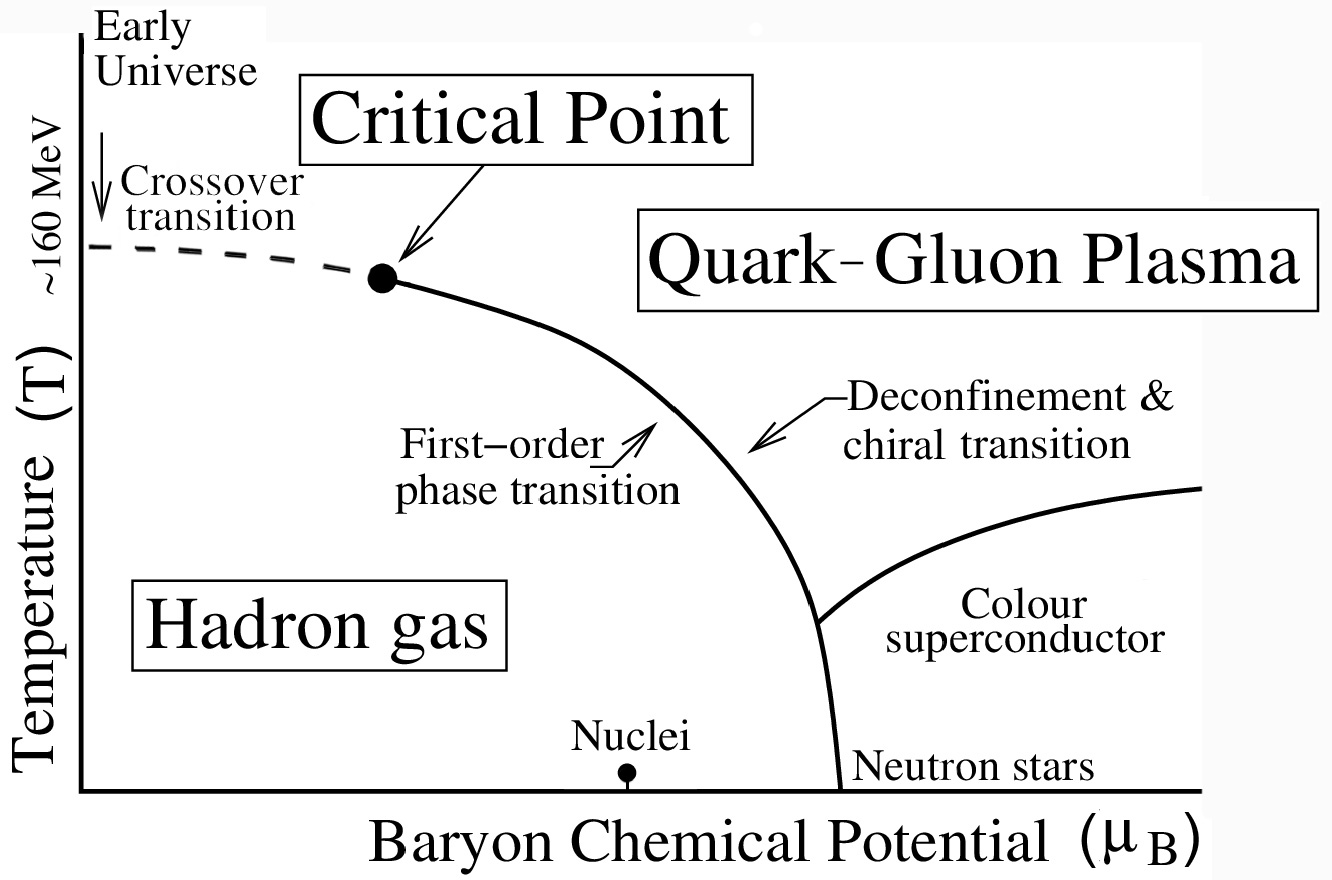
\includegraphics[width=0.8\textwidth]{figures/png/phase_diagram.jpg}
    \caption{The QCD phase diagram.}\label{fig:phase_diagram}
\end{figure}

\section{Heavy Ion Collisions}

Heavy ion collisions produce conditions similar to the very early universe, forming the QGP along with many other processes. A collision undergoes several stages starting from the moments before the collision, to the final state of the collision that is measured by our detectors. These stages are useful for organizing computations and simulations of the collision, as well as characterizing the modifications that the presence of a QGP has on each stage. In this analysis we focus on Pb-Pb collisions, but other species have been collided at the Large Hadron Collider (LHC) and the Relativistic Heavy Ion Collider (RHIC).

\subsection*{Initial State}

The initial state of a Pb-Pb collision is characterized by the transverse spatial distribution, and the longitudinal momentum distribution of each parton in the colliding nuclei, described by the Glauber model and nuclear parton distribution function (PDF) respectively. The Glauber model approximates the nuclei as a collection of nucleons, which are transversely distributed in the nucleus according to a Woods-Saxon distribution and follow a straight trajectory. 

\subsection*{QGP}

\subsection*{Hydrodynamic Evolution}

\subsection*{Hadronization}

\subsection*{Chemical Freeze-Out}

\subsection*{Thermal Freeze-Out}

\section{Jets}

Introductory paragraph about jets and why they are used as tools of internal tomography in the QGP
%TODO: Expand with a bit more theory

\subsection*{Jet Reconstruction}

Jet-finding algorithms are designed to group objects together into jets based on their kinematic properties in both theoretical simulations and measured data. Simulations provide access to complete information about the underlying physics and is not subject to experimental limitations. Therefore, to facilitate comparison with theoretical calculations, jet-finding algorithms are designed to be infrared and collinear safe, ensuring that their properties remain calculable in perturbative QCD. There are a number of different algorithms for reconstructing jets, including the anti-$k_T$ algorithm~\cite{antiKt}, the $k_T$ algorithm~\cite{kT}, and the Cambridge-Aachen algorithm~\cite{FastJet}, which all fall into the class of sequential recombination algorithms introduced for hadron colisions in~\cite{seq_rec}. The anti-$k_T$ algorithm is used in this analysis. The anti-$k_T$ algorithm is infrared and collinear safe.

\subsubsection*{Anti-$k_T$ Algorithm}
The anti-$k_T$ algorithm begins by defining a list of entities, either particles, tracks, detector hits, or groups of these referred to as pseudojets that are used to construct the jets. The algorithm proceeds by sequentially and recursively grouping entities until every entity is assigned to a psuedojet and then marked as a jet.  The anti-$k_T$ algorithm defines a distance measure between two entities, $d_{ij}$, and between an entity and the beam, $d_{iB}$. The distance measure is defined as

\begin{equation}
d_{ij} = \min(p_{Ti}^{-2} p_{Tj}^{-2})\frac{\Delta_{ij}^2}{R^2}
\end{equation}

where $p_{Ti}$ and $p_{Tj}$ are the transverse momenta of entities i and j, respectively, $\Delta_{ij}^2$=$(\eta_i - \eta_j )^2$ + $(\phi_i - \phi_j )^2$, and R is the radius parameter, whose particular value is chosen as part of the definition of the analysis. The distance measure between an entity and the beam is defined as

\begin{equation}
d_{iB} = p_{Ti}^{-2}
\end{equation}

The anti-$k_T$ algorithm then finds the minimum of ${d_{ij}, d_{iB}}$ for each entity i. If the minimum is $d_{ij}$, then entities i, and j are combined into a pseudojet with a four-momentum given by the sum of the four-momenta of entities i and j. If the minimum is $d_{iB}$, then entity i is labeled as a jet and removed from the list of entities. The anti-$k_T$ algorithm then repeats the process until there are no entities left in the list of entities.

The anti-$k_T$ algorithm tends to cluster higher momentum particles first which reduces the effects of the underlying event and pile-up. However, the anti-$k_T$ algorithm also clusters all the particles in an event, including those which arise from the underlying event and pile-up. This means that the resulting population of jets is contaminated by the presence of combinatorial jets which are not associated with any hard scattering process of interest. There are various techniques for supressing combinatorial jets, and the correct choice depends heavily on the type of analysis being performed. In our analysis, the presence of combinatorial jets confuses the interpretation of the results, so we apply liberal cuts to reduce their presence in our sample. 

The other secquential recombination algorithms, $k_T$ and Cambridge-Aachen, have other strengths and weaknesses. The simple difference between these algorithms is the definition of the distance measure. The $k_T$ algorithm defines the distance measure as

\begin{equation}
d_{ij} = \min(p_{Ti}^{2} p_{Tj}^{2})\frac{\Delta_{ij}^2}{R^2}
\end{equation}

and the Cambridge-Aachen algorithm defines the distance measure as

\begin{equation}
d_{ij} = \frac{\Delta_{ij}^2}{R^2}.
\end{equation}

The $k_T$ algorithm tends to cluster softer particles first, which typically arise from the underlying event. The Cambridge-Aachen algorithm clusters particles based on their angular separation, which is useful in measurements of the substructure of jets. The $k_T$ algorithm is used in this analysis to estimate the background density. 

\subsubsection*{Jet Area}
Jet areas provide a measure of the extent of a jet in the $\eta$-$\phi$ plane. The jet area is estimated by filling an event with many very soft particles, called ghosts, and clustering them into jets. The jet area is then proportional to the number of ghosts that are clustered into that jet. A jet's area is closely related to its senstitivity to soft background contamination and is used to estimate the background contamination in that jet. 

\subsubsection*{Charged and Full Jets} 
Jets are composed of charged and neutral hadrons. In experiment, we have much more precise information about the charged hadrons in jets due to the types of detectors we use. Experimentally, therefore, we make the distinction between charged and full jets, the former composed only of charged hadrons and the latter composed of charged and neutral hadrons. Charged hadrons are measured using the detectors in the central barrel of ALICE, which have full geometric coverage and excellent momentum resolution.  The neutral hadrons can only be measured in the calorimeter which has limited geometric coverage and a lower momentum resolution at low momentum which improves towards higher momentum. Measurements of charged and full jets are complementary, but differ in their relation to theoretical calculations. Charged jets are missing their neutral component and so their properties are not directly calculable in perturbative QCD, but their measurements are more precise than full jets and can still be used to constrain theoretical calculations. The properties of full jets are directly calculable in perturbative QCD, but their measurements are less precise. In this analysis, we use full jets for a more direct comparison to theoretical calculations.

\subsection*{Factorization Theorem}

\subsection*{Medium Modification}

\subsection*{Jet Quenching}

\subsection*{Hadronization Modification}

\section{Previous Results}

\begin{enumerate}
    \item Hadron $R_{AA}$
    \item Jet $R_{AA}$
    \item $v_2$-inclusive and jet
    \item Jet Modification
    \item PID Jet Results
\end{enumerate}